\label{sec:data}

\subsection{Synthetic Data Generation}

The generator produces structured CSV records covering 13 Windows Event IDs relevant to
the ICS threat model (Table~\ref{tab:eventids}). Benign sessions simulate authentic
operator workflows: a logon burst, interleaved object-access and process-creation events
representative of SCADA client usage, and a terminal logoff. Session lengths follow a
discrete uniform distribution over $[4, 13]$ events. Inter-event gaps follow
$\text{Uniform}(5, 300)$~seconds, reflecting operator think-time.

\begin{table}[!t]
  \caption{Windows Event IDs Used in the Dataset}
  \label{tab:eventids}
  \centering
  \begin{tabular}{clc}
    \hline
    Event ID & Description & Label \\
    \hline
    4624 & Account logon success     & B/M \\
    4625 & Account logon failure     & B/M \\
    4634 & Account logoff            & B   \\
    4648 & Explicit credentials logon & B  \\
    4663 & Object access attempt     & B/M \\
    4656 & Object handle requested   & B   \\
    4672 & Special privileges assigned & M  \\
    4688 & New process created       & B/M \\
    4689 & Process exited            & B/M \\
    4720 & User account created      & B   \\
    4732 & Group membership change   & B   \\
    7045 & Service installed         & M   \\
    7036 & Service state change      & M   \\
    \hline
    \multicolumn{3}{l}{\footnotesize B = benign, M = malicious, B/M = both}
  \end{tabular}
\end{table}

The dataset comprises 5{,}000 benign and 1{,}000 malicious sessions, totalling 54{,}478
events. The 5:1 class ratio reflects a realistic operational environment in which malicious
sessions are rare. Smart grid hostnames follow SCADA~HMI, RTU~CTRL, \texttt{eng\_station},
and \texttt{historian} naming conventions. All sessions carry a \texttt{session\_id} UUID
for group-level train/val/test splitting.

\subsection{Feature Engineering Pipeline}

Figure~\ref{fig:featpipe} illustrates the five feature groups extracted per session.

\begin{figure}[!t]
  \centering
  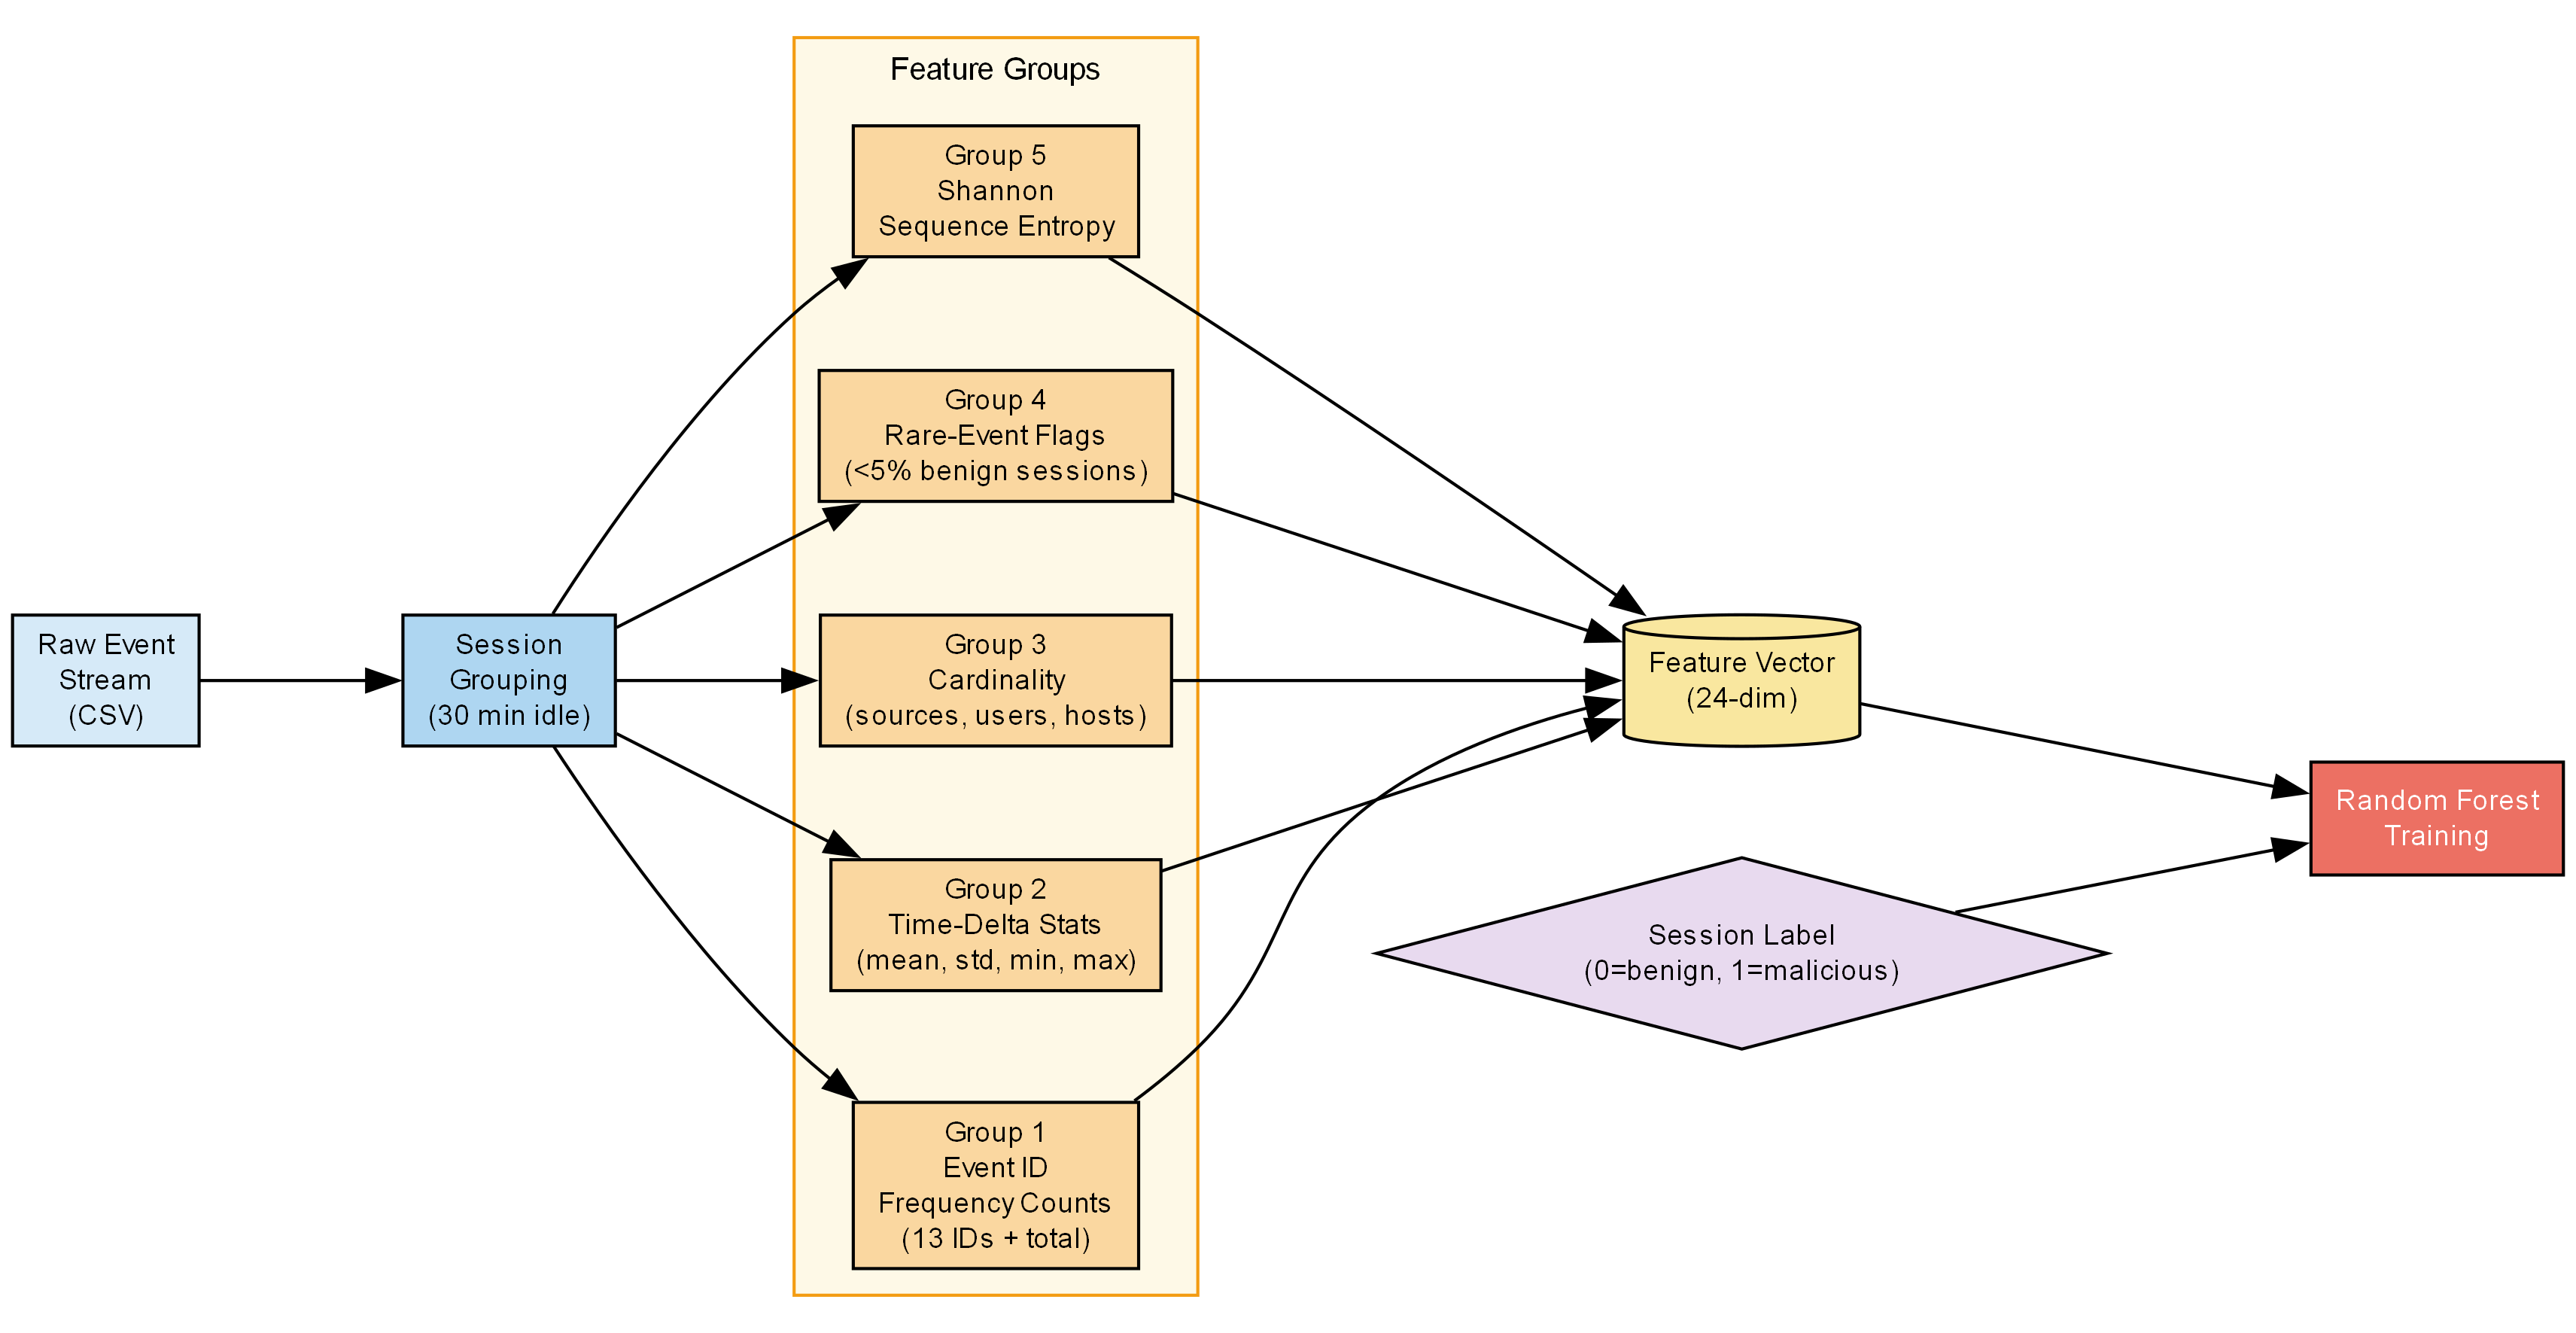
\includegraphics[width=\columnwidth]{figs/feature_pipeline.png}
  \caption{Feature engineering pipeline: five groups extracted from each session.}
  \label{fig:featpipe}
\end{figure}

\subsubsection{Group~1: Event Frequency Counts}
For each of the 13 event IDs in Table~\ref{tab:eventids} plus a total-event counter,
we compute the raw occurrence count within the session. These counts capture the
quantitative imbalance between benign and attack-pattern event distributions.

\subsubsection{Group~2: Time-Delta Statistics}
Let $\{t_1, t_2, \ldots, t_n\}$ be event timestamps sorted ascending. We compute
$\Delta_i = t_{i+1} - t_i$ (in seconds) and extract $\{\text{mean}(\Delta), \text{std}(\Delta),
\min(\Delta), \max(\Delta)\}$. Reconnaissance and lateral-movement attacks exhibit
anomalously small $\min(\Delta)$ and $\text{mean}(\Delta)$ compared to benign sessions.

\subsubsection{Group~3: Host and User Cardinality}
Counts of unique \texttt{source} (IP or hostname), \texttt{user}, and \texttt{hostname}
values within a session serve as lateral-spread indicators. Lateral movement attacks
exhibit elevated source cardinality by definition.

\subsubsection{Group~4: Rare-Event Flags}
An event ID is flagged as rare if it appears in fewer than 5\% of benign training sessions.
Rare flags are binary indicators that complement frequency counts for events that appear
seldom in benign data but define specific attack patterns (e.g., event~7045 in the
persistence attack).

\subsubsection{Group~5: Sequence Entropy}
Shannon entropy $H = -\sum_{e} p(e) \log_2 p(e)$ over the empirical event-ID distribution
measures diversity of event types. Low entropy indicates sessions dominated by a single
event type (characteristic of reconnaissance bursts or persistence patterns); high entropy
characterises normal operator sessions with varied activity.

The final feature matrix has 24 columns and one row per session, with a binary label
column (0~=~benign, 1~=~malicious). Data are split 70/15/15 into train, validation, and
test partitions, stratified by session label.
